\documentclass[a4paper, 12pt, final, garamond]{book}
%\usepackage{cours-preambule}
\usepackage{bpep_full}
\usepackage{chngcntr}

\counterwithin*{equation}{section}
\counterwithin*{equation}{subsection}

\raggedbottom

\makeatletter
\renewcommand{\@chapapp}{\'Electrocin\'etique -- chapitre 4}
\makeatother

\begin{document}
\setcounter{chapter}{3}

\renewcommand{\f}[2]{{
		\mathchoice
		{\dfrac{#1}{#2}}
		{\dfrac{#1}{#2}}
		{\frac{#1}{#2}}
		{\frac{#1}{#2}}
}}

\newcommand{\e}[1]{{}_{\text{#1}}}

\toggletrue{corrige}  % décommenter pour passer en mode corrigé

\resetQ
\chapter{\sujetUniquement{TD~: oscillateurs harmonique et amorti}\siCorrige{Correction du TD}}

\resetQ
\subimport{/home/nicolas/Documents/Enseignement/Prepa/bpep/exercices/TD/RLC_transitoire_QCM/}{sujet.tex}

\resetQ
\subimport{/home/nicolas/Documents/Enseignement/Prepa/bpep/exercices/TD/transitoire_RLC/}{sujet.tex}

\resetQ
\section{Masse percutant un ressort}

\begin{minipage}{0.70\linewidth}

    Un ressort (raideur $k$ et longueur à vide $\ell_0$) fixé en $O$ est initialement au
    repos. Une masse $m$ glisse sans frottement à vitesse constante $\vv{v} =
    -v_0\vv*{u}{x}$ avec $v_0 > 0$
    et s'accroche \textit{définitivement} au ressort à l'instant $t = 0$.
\end{minipage}
\hfill
\begin{minipage}{0.3\linewidth}
    \centering
    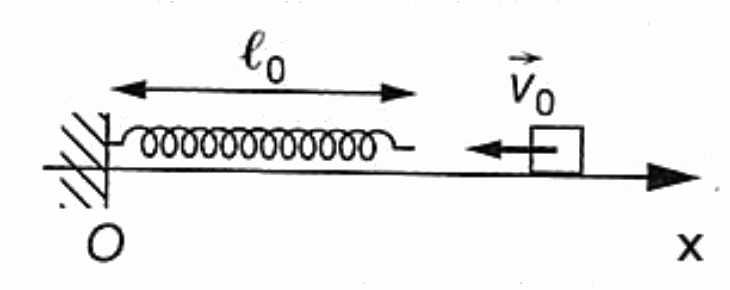
\includegraphics[width=\linewidth]{ressort_v0}
\end{minipage}

\QR{Déterminer l'équation du mouvement de la masse une fois qu'elle est
accrochée (pour $t \geq 0$). }{Une fois la masse accrochée, on retrouve la
    situation du cours. On fait le bilan des forces~:
    \[ \begin{array}{ll}
        \textbf{Poids} & \Pf = -mg\uy\\
        \textbf{Support} & \Rf = R\uy\\
        \textbf{Ressort} & \Ff = -k(\ell - \ell_0)\ux
    \end{array}\]
    On effectue le changement de variable $x = \ell -\ell_0$, et avec le PFD on
    a donc
    \begin{gather*}
        m\af = \Pf + \vv{R} + \Ff\\
        \Leftrightarrow m\left(
            \begin{array}{c}
                \dv[2]{x}{t}\\
                0
            \end{array}
        \right)
        =
        \left(
            \begin{array}{c}
                -kx\\
                -mg + R
            \end{array}
        \right)
    \end{gather*}
    Sur l'axe $\ux$ on trouve bien 
    \begin{equation*}
        \boxed{m \dv[2]{x}{t} + kx = 0} \Leftrightarrow \boxed{ \dv[2]{x}{t} +
        \w_0{}^2x = 0}
    \end{equation*}
    avec $\w_0 = \sqrt{\dfrac{k}{m}}$. La projection sur $\uy$ montre que la
réaction du support compense le poids.}

\QR{Résoudre cette équation en tenant compte des conditions initiales.
}{À $t=0$, la masse est accrochée au ressort de longueur $\ell_0$ et elle arrive
    avec $\vf(0) = -v_0\ux$. On a donc
    \begin{equation*}
        \boxed{x(0) = 0}\qet\boxed{ \dv{x}{t} (0) = -v_0}
    \end{equation*}
    La forme générale de la solution est
    \[ \boxed{x(t) = A\cos(\w_0t) + B\sin(\w_0t)}\]
    Avec conditions initiales,
    \begin{gather*}
        x(0) = A\underbrace{\cos(0)}_{=1} + B\underbrace{\sin(0)}_{=0}
        \Leftrightarrow A = 0\\
        \dv{x}{t} (0) = -A\w_0\underbrace{\sin(0)}_{=0} +
        B\w_0\underbrace{\cos(0)}_{=1} \Leftrightarrow B = - \frac{v_0}{\w_0}
    \end{gather*}
    On a donc
    \begin{equation*}
        \boxed{x(t) = -\frac{v_0}{\w_0}\sin(\w_0t)}
    \end{equation*}
}

\QR{À quelle condition la masse vient-elle percuter la paroi en O~?}{
    En supposant que le ressort puisse se comprimer à l'infini, la masse vient
percuter la paroi située en $O$ si l'amplitude de $x$ est égale à $-\ell_0$,
c'est-à-dire
\[\boxed{\frac{v_0}{\w_0} = \ell_0} \Leftrightarrow \boxed{v_0 = \w_0\ell_0}\]
On remarque donc que plus $v_0$ est grande, plus cela est facile, mais également
que plus $\w_0$ est faible est plus cela est facile. En effet, plus la pulsation
est élevée et moins la masse a d'amplitude à $v_0$ fixée. Ceci correspond bien à
l'intuition qu'on pourrait en avoir énergétiquement~: une énergie mécanique
totale se répartit dans l'énergie potentielle élastique d'une part, c'est-à-dire
la distance d'élongation du ressort, et dans l'énergie cinétique d'autre part,
donc dans sa vitesse.}

\resetQ
\section{Oscillateur à deux ressorts}

Un mobile supposé ponctuel de masse $m$ est astreint à glisser le long d'une
tige horizontale de direction $(Ox)$. Ce mobile est relié par deux ressort
linéaires à deux points fixes $A$ et $B$. On le repère par sa position $OM = x$.

\begin{center}
    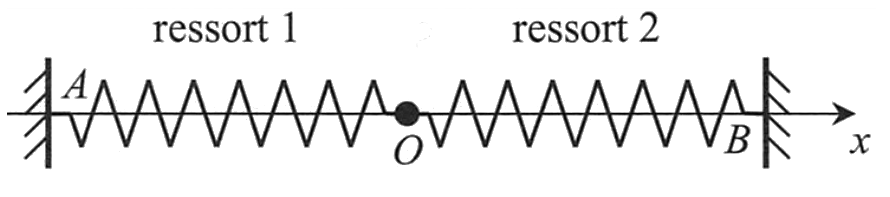
\includegraphics[width=.5\linewidth]{ressort_double}
\end{center}

Les deux ressorts sont identiques~: même constante de raideur $k$ et même
longueur au repos $\ell_0$. Dans la position d'équilibre du système, les
longueurs des ressorts sont identiques et valent $\ell_{\rm eq}$ et le mobile se
trouve à l'origine $O$ de l'axe. On se place dans le référentiel terrestre (lié
au sol), considérée comme galiléen. À $t = 0$, le mobile est abandonné sans
vitesse initiale d'une position $x_0 \neq 0$

\QR{Dans un premier temps, on néglige tout frottement.
    \begin{enumerate}
        \item Établir l'équation différentielle vérifiée par $x(t)$.
        \item Montrer que le système constitue un oscillateur harmonique dont on
            précisera la pulsation $\w_0$ et la période $T_0$ propres en
            fonction de $k$ et $m$.
        \item Donner l'expression de $x(t)$ en tenant compte des conditions
            initiales.
    \end{enumerate}
}{
    \begin{enumerate}
        \item Cette fois-ci, on a deux ressorts~: le premier tire dans le sens
            $-\ux$ et le second dans le sens $+\ux$~; ainsi le bilan des forces
            s'exprime~:
            \[ \begin{array}{ll}
                \textbf{Poids} & \Pf = -mg\uy\\
                \textbf{Support} & \Rf = R\uy\\
                \textbf{Ressort 1} & \Ff_1 = -k(\ell_1 - \ell_0)\ux = -k (\ell_{\rm
                eq} + x - \ell_0)\ux\\
                    \textbf{Ressort 2} & \Ff_2 = +k(\ell_2 - \ell_0)\ux = +k (\ell_{\rm
                eq} - x - \ell_0)\ux
            \end{array}\]
            On a en effet $\ell_1$ la longueur du ressort 1 qui s'exprime
            $\ell_1 = \obar{AM}$. Or, d'après l'énoncé $\ell_{\rm eq} = AO =
            OB$~: en décomposant, on a donc $\obar{AM} = \obar{AO} + \obar{OM} =
            \ell_{\rm eq} + x$. Le ressort 2 a comme longueur $\ell_2 =
            \obar{MB} = \obar{MO} + \obar{OB}$ soit $\ell_2 = \ell_{\rm eq} -
            x$.\smallbreak
            Ainsi, le PFD donne
            \begin{gather*}
                m\af = \Pf + \Rf + \Ff_1 + \Ff_2\\
                \Leftrightarrow m\left(
                    \begin{array}{c}
                        \dv[2]{x}{t}\\
                        0
                    \end{array}
                \right)
                =
                \left(
                    \begin{array}{c}
                        -k(\bcancel{\ell_{\rm eq}} + x - \cancel{\ell_0})
                        +k(\bcancel{\ell_{\rm eq}} - x -\cancel{\ell_0})\\
                        -mg + R
                    \end{array}
                \right)
            \end{gather*}
            Sur l'axe $\ux$ on trouve
            \begin{equation*}
                \boxed{m \dv[2]{x}{t} + 2kx = 0} \Leftrightarrow \boxed{\dv[2]{x}{t} +
                \frac{2k}{m}x = 0}
            \end{equation*}
            La projection sur $\uy$ montre que la réaction du support compense
            le poids.
        \item Sous forme canonique, cette équation se réécrit
            \begin{equation*}
                \boxed{ \dv[2]{x}{t} + \w_0{}^2x = 0}
            \end{equation*}
            C'est bien l'équation d'un oscillateur harmonique de pulsation
            \fbox{$\w_0 = \sqrt{\dfrac{2k}{m}}$} et donc de période \fbox{$T_0 =
            \dfrac{2\pi}{\w_0} = 2\pi \sqrt{\dfrac{m}{2k}}$}. Doubler la
            constante de raideur divise par $\sqrt{2}$ la période~: le ressort
            oscille plus vite qu'avec un seul ressort.
        \item L'expression générale de $x(t)$ est donc $x(t) = A\cos(\w_0t) +
            B\sin(\w_0t)$. Or, en $t=0$, on a $x(0) = x_0 = A$, et $ \dv{x}{t}
            (0) = 0 = \w_0 B$~; ainsi
            \begin{equation*}
                \boxed{x(t) = x_0\cos(\w_0t)}
            \end{equation*}
    \end{enumerate}
}

\QR{En fait il existe entre le mobile et la tige un frottement de type visqueux
    linéaire, la force de frottement s'exprime $\vv{F} = -\alpha\vv{v}$ (avec
    $\alpha > 0$ et $\vv{v}$ la vitesse de la masse $m$ dans le référentiel
    terrestre).
    \begin{enumerate}
        \item Établir l'équation différentielle vérifiée par $x(t)$. On posera
            $h = \dfrac{\alpha}{m}$.
        \item Montrer que lorsque $\alpha < 2^{3/2}\sqrt{km}$, le mouvement
            comporte des oscillations amorties. Donner l'expression de $x(t)$ en
            tenant compte des conditions initiales et exprimer la pseudo-période
            $T$ en fonction de $\w_0$ et $h$.
    \end{enumerate}
}{
    \begin{enumerate}
        \item On ajoute $\vv*{F}{\rm frott} = -\alpha v\ux$ au PFD, ce qui donne
            \[ \boxed{ \dv[2]{x}{t} + h \dv{x}{t} + \w_0{}^2x = 0}\]
        \item On sait qu'on a des oscillations amorties quand le discriminant
            $\Delta$ de l'équation caractéristique est négatif~: $\Delta < 0$.
            Or ici, l'équation caractéristique est
            \begin{gather*}
                r^2 + hr + \w_0{}^2 = 0 \Rightarrow \Delta = h^2 - 4\w_0{}^2\\
                \Delta < 0 \Leftrightarrow
                \left(\frac{\alpha}{m}\right)^{\cancel{2}} <
                \underset{2}{\cancel{4}}\w_0{}^{\cancel{2}} \Leftrightarrow \alpha < 2m
                \sqrt{\frac{2k}{m}}\\
                \Leftrightarrow \alpha < 2^{3/2} \sqrt{km}
            \end{gather*}
            Dans ce régime, on aura donc les racines
            \begin{gather*}
                r_\pm = - \frac{h}{2} \pm \Ir \sqrt{\w_0{}^2 - \frac{h^2}{4}}
                \Leftrightarrow \boxed{r_\pm = - \frac{h}{2} \pm \Ir\w} \qavec
                \boxed{\w = \sqrt{\w_0{}^2 - \frac{h^2}{4}}}
            \end{gather*}
            La solution générale est alors
            \[ \boxed{x(t) = \exr^{-ht/2} \left[ D\cos(\wt) + E\sin(\wt) \right]}\]
            On a les mêmes conditions initiales, soit $x(0) = x_0 = D$ et $
            \dv{x}{t} (0) = 0 = - \frac{h}{2}x_0 + \w E$, d'où $E =
            \frac{h}{2\w}x_0$. Ainsi,
            \begin{equation*}
                \boxed{x(t) = x_0\exr^{-ht/2} \left[ \cos(\wt) +
                \frac{h}{2\w}\sin(\wt) \right]}
            \end{equation*}
            On a donc une pseudo-période \fbox{$T = \dfrac{2\pi}{\w} =
            \dfrac{2\pi}{\sqrt{\w_0{}^2 - \frac{h^2}{4}}}$}
    \end{enumerate}
}

\resetQ
\section{Décrément logarithmique électrique}
On étudie la réponse $u(t)$ à un échelon de tension $e(t)$ tel que
$ \left\{
        \begin{array}{rcl}
            e(t<0)    & = & 0 \\
            e(t\geq0) & = & E
        \end{array}
\right.$
dans le circuit ci-dessous.

\begin{center}
    \switch{
    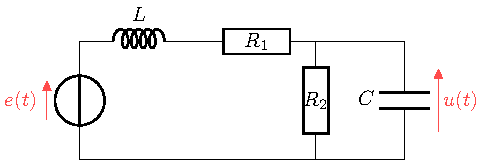
\includegraphics[width=.5\linewidth]{dec_log-plain}}{
    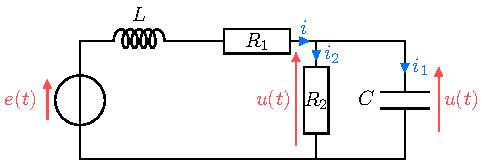
\includegraphics[width=.5\linewidth]{dec_log-intens}
}
\end{center}

\QR{Déterminer la valeur $u_{\infty}$ vers laquelle tend $u(t)$ lorsque $t
        \longrightarrow \infty$.
}{$R_2$ et $C$ sont en parallèle, donc $u(t)$ est à la fois la tension aux
    bornes de $C$ et de $R_2$. De plus, à $t \longrightarrow \infty$, la bobine
    se comporte comme un fil et le condensateur comme un interrupteur ouvert. Le
    circuit est donc équivalent à un diviseur de tension avec $R_1$ et $R_2$ en
série alimentées par la tension $e(t)$, et on a donc
\[ \boxed{u(\infty) = u_{\infty} = \frac{R_2}{R_1 + R_2}E}\]}

\QR{Montrer que $\DS \dv[2]{u}{t} + 2\lambda \dv{u}{t} +\w_0{}^2 u =
    \w_0{}^2u_{\infty}$. Exprimer $\lambda$ et $\w_0$ en fonction de $L$, $C$,
    $R_1$ et $R_2$.
}{
    Avec une loi des mailles et les relations courant-tension~:
    \[ u + L \dv{i}{t} + R_1i = E\]
    Avec la loi des nœuds~:
    \begin{gather*}
        i = i_1 + i_2 = C \dv{u}{t} + \frac{u}{R_2}
    \end{gather*}
    En combinant~:
    \begin{gather*}
        u + L \dv{}{t} \left( C \dv{u}{t} + \frac{u}{R_2} \right) + R_1C
        \dv{u}{t} + R_1\frac{u}{R_2} = E\\
        \Leftrightarrow u + LC \dv[2]{u}{t} + \frac{L}{R_2} \dv{u}{t} +
            R_1C \dv{u}{t} + \frac{R_1}{R_2}u = E\\
        \Leftrightarrow LC \dv[2]{u}{t} + \left( \frac{L}{R_2} + R_1C 
        \right)\dv{u}{t} + \left( \frac{R_1}{R_2} + \underset{
            \frac{R_2}{R_2}}{\cancel{1}} \right)u = E\\
        \Leftrightarrow \dv[2]{u}{t} + \left( \frac{1}{R_2C} + \frac{R_1}{L}
            \right) \dv{u}{t} + \left( \frac{R_1 + R_2}{R_2} \right) \frac{u}{LC} =
            \frac{E}{LC}\\
        \Leftrightarrow \dv[2]{u}{t} + \left( \frac{1}{R_2C} + \frac{R_1}{L}
            \right) \dv{u}{t} +\left( \frac{R_1 + R_2}{R_2} \right)
            \frac{u}{LC} = \left(\frac{R_1 + R_2}{R_2}\right)
            \frac{u_{\infty}}{LC}\\
        \Leftrightarrow \boxed{\dv[2]{u}{t} + 2\lambda \dv{u}{t} + \w_0{}^2u =
            \w_0{}^2u_\infty}\\
            \text{avec} \quad \boxed{\w_0 = \sqrt{\frac{1}{LC} \left( \frac{R_1 +
        R_2}{R_2} \right)}} \qet \boxed{\lambda = \frac{1}{2} \left(
\frac{1}{R_2C} + \frac{R_1}{L} \right)}
    \end{gather*}
}

\QR{On observe à l'oscilloscope la courbe $u(t)$ ci-contre.

    \begin{minipage}{0.6\linewidth}
        \begin{enumerate}
            \item Déterminer la valeur numérique de la pseudo-période $T$.
            \item Déterminer la valeur numérique du décrément logarithmique
                \[\boxed{ \delta = \frac{1}{n} \ln \left( \frac{u(t) -
                u_{\infty}}{u(t+nT)-u_{\infty}} \right)}\]
        \end{enumerate}
    \end{minipage}
    \begin{minipage}{0.4\linewidth}
        \centering
        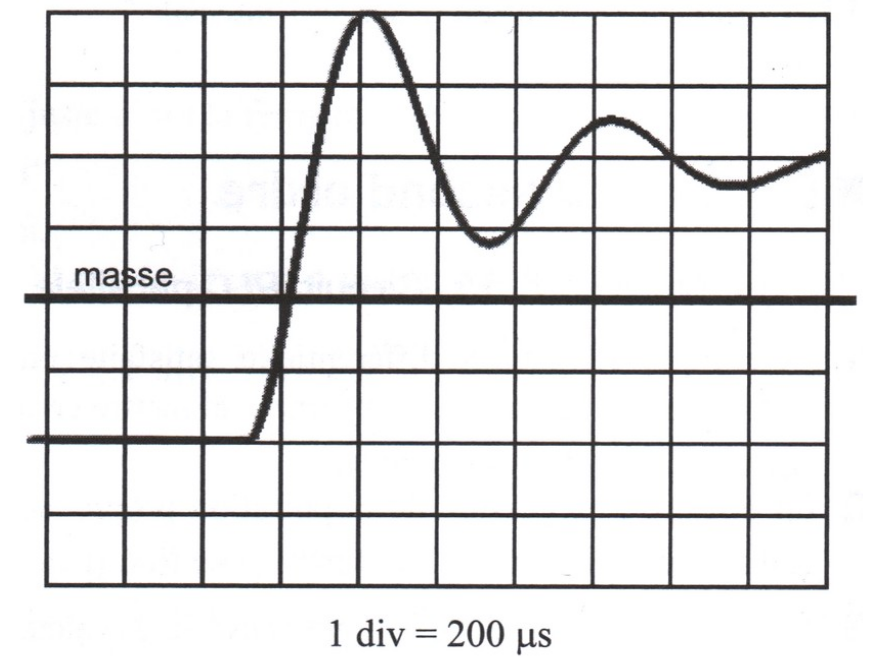
\includegraphics[width=\linewidth]{dec_log-courbe}
    \end{minipage}
}{
    \begin{enumerate}
        \item On a un régime pseudo-périodique, où on lit que \fbox{$T =
            \SI{600}{\micro s}$}.
        \item On ne peut calculer $\delta$ qu'avec une pseudo-période ici. On
            lit au premier pic à $t_1$ la valeur de la tension \textbf{par
            rapport à la masse}~: $u(t_1) =
            \SI{4}{V}$. Au second pic à $t_2 = t_1 + T$ on a~: $u(t_1 + T) =
            \SI{2.5}{V}$. De plus, $u_\infty = \SI{2}{V}$. Ainsi,
            \begin{equation*}
                \boxed{\delta = \ln \left( \frac{4 - 2}{2.5-2} \right) = \ln(4)
                = \num{1.39}}
            \end{equation*}
    \end{enumerate}
}

\QR{Exprimer $u(t)$ en fonction de $u_{\infty}$, $\w_0$, $\lambda$ et $t$ (sans
chercher à déterminer les constantes d'intégration).
}{
    Pour la solution de l'équation homogène, on cherche les racines du polynôme
    caractéristique de discriminant $\Delta$~:
    \begin{gather*}
        r^2 + 2\lambda r + \w_0{}^2 = 0 \Rightarrow \Delta = 4(\lambda^2 - \w_0{}^2)
    \end{gather*}
    On sait que $\Delta < 0$ puisqu'on observe des oscillations amorties. On
    aura donc
    \begin{gather*}
        r_\pm = -\frac{\cancel{2}\lambda}{\cancel{2}} \pm \Ir
            \frac{1}{\bcancel{2}}\sqrt{\bcancel{4}(\w_0{}^2 - \lambda^2)}
        \Leftrightarrow
        \boxed{r_\pm = -\lambda \pm \Ir \w}
            \qavec
        \boxed{\w = \sqrt{\w_0{}^2 - \lambda^2}}
    \end{gather*}
    La solution particulière étant visiblement $u_\infty$, on aura la forme
    générale
    \begin{equation*}
        \boxed{u(t) = \exr^{-\lambda t} \left( A\cos\wt + B\sin\wt \right) +
        u_\infty}
    \end{equation*}
}

\QR{Déterminer la relation entre $\delta$, $\lambda$ et $T$. En déduire la
valeur numérique de $\lambda$.
}{
    Avec l'expression de $u(t)$, on peut développer le dénominateur de
    $\delta$~:
    \begin{gather*}
        u(t+nT) - u_\infty = \exr^{-\lambda nT}\times
            \underbrace{\exr^{-\lambda t}
            \left(
                A\underset{=\cos\wt}{\underline{\cos(\wt+n\wt)}} +
                B\underset{=\sin\wt}{\underline{\sin(\wt+n\wt)}}\right)
            }_{u(t) - u_\infty}
    \end{gather*}
    Ainsi,
    \begin{gather*}
        \frac{u(t) - u_\infty}{u(t+nT)-u_\infty} = \exr^{+\lambda nT}
        \Rightarrow
        \delta = \frac{1}{n} \ln (\exr^{\lambda nT})\\
        \Leftrightarrow \boxed{\delta = \lambda T \Leftrightarrow \lambda =
        \frac{\delta}{T}} \qavec \left\{
            \begin{array}{rcl}
                \delta & = & \num{1.39}\\
                T & = & \SI{600}{\micro s}
            \end{array}
        \right.\\
        \text{A.N.~:~}\boxed{\lambda = \SI{2.32e3}{s^{-1}}}
    \end{gather*}
}
    
\QR{Sachant que $R_1 = \SI{200}{\ohm}$, $R_2 = \SI{5}{k\ohm}$ et $L =
\SI{500}{mH}$, déterminer la valeur de $C$.
}{
    On sait que $\lambda$ s'exprime en fonction de $C$, on l'isole donc de son
    expression~:
    \begin{gather*}
        2\lambda = \frac{1}{R_2C} + \frac{R_1}{L}
        \Leftrightarrow
        R_2C = \frac{1}{2\lambda - \frac{R_1}{L}}\\
        \Leftrightarrow \boxed{C = \frac{1}{2R_2\lambda - \frac{R_1R_2}{L}}}
        \qavec
        \left\{
            \begin{array}{rcl}
                R_1 & = & \SI{200}{\ohm}\\
                R_2 & = & \SI{5}{k\ohm}\\
                L & = & \SI{500}{mH}\\
                \lambda & = & \SI{2.32e3}{s^{-1}}
            \end{array}
        \right.\\
        \text{A.N.~:~} \boxed{C = \SI{76}{\micro F}}
    \end{gather*}
}
\siCorrige{
    \begin{impo}[label=impo:declog]{À retenir}
        En régime pseudo-périodique, l'amortissement du signal est dû à
        l'exponentielle de la solution générale. En calculant le logarithme du
        rapport de la solution à un instant $t$ et de la solution à un instant
        $t+nT$ avec $T$ la période on calcule donc le facteur de l'exponentielle
        décroissante, ce qui permet de trouver les caractéristiques du circuit.
    \end{impo}
}

\resetQ
\section{Décrément logarithmique mécanique}

\begin{minipage}{0.49\linewidth}
    Une masse $m$ est accrochée à un ressort de raideur $k = \SI{10}{N.m^{-1}}$
    et de longueur à vide $\ell_0 = \SI{10}{cm}$, fixé au point $O$. En plus de
    son poids et de la force de rappel du ressort, la masse est soumise à une
    force de frottement fluide $\Ff = -\alpha\vv{v}$. Un capteur fournit l'évolution
    de $u(t) = z(t)−z_{\rm eq}$ au court du temps.
\end{minipage}
\begin{minipage}{0.49\linewidth} \centering
    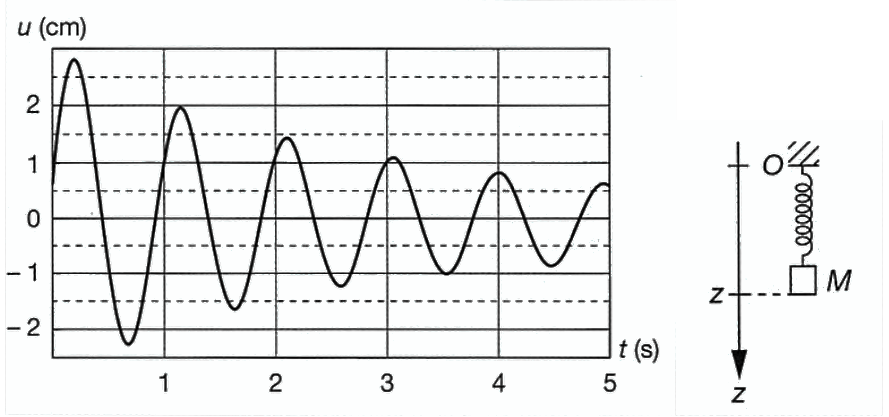
\includegraphics[width=\linewidth]{dec_log-courbe_meca}
\end{minipage}

\QR{Établir l'équation d'évolution de $z(t)$. Quelle est la position d'équilibre
    $z_{\rm eq}$ de la masse ? En déduire une équation satisfaite par $u(t)$.
}{On repère par $z$ l'altitude du ressort. Étant donné le système, le mouvement
    ne s'effectue que selon $\uz$, et on a $v = \dv{z}{t}$ et $a =
    \dv[2]{z}{t}$. De plus, la longueur $\ell$ du ressort s'identifie à
    l'altitude $z$ de la masse. On effectue donc le \textbf{bilan des forces} en
    faisant attention au sens de $\uz$~:
    \[ \begin{array}{ll}
        \textbf{Poids} & \Pf = mg\uz\\
        \textbf{Ressort} & \vv*{F}{\rm ressort} = -k (z-\ell_0)\uz\\
        \textbf{Frottement} & \Ff = -\alpha \dv{z}{t}\uz
    \end{array}\]
    Ainsi, le \textbf{PFD} donne
    \begin{gather*}
        m \dv[2]{z}{t} = mg - k(z-\ell_0) -\alpha \dv{z}{t}
        \Leftrightarrow
        \boxed{m\dv[2]{z}{t} + \alpha \dv{z}{t} + kz = mg + k\ell_0}
    \end{gather*}
    À l'équilibre, $\dv{z}{t} = 0$ et $\dv[2]{z}{t} = 0$, on trouve donc
    \begin{equation*}
        z_{\rm eq} = \ell_0 + \frac{mg}{k}
    \end{equation*}
    À cause du poids qui n'est cette fois pas compensé par la réaction du
    support, la longueur d'équilibre est plus grande que la longueur à vide du
    ressort. On réexprime l'équation différentielle avec le changement de
    variable de l'énoncé pour avoir
    \begin{gather*}
        \boxed{m\dv[2]{u}{t} + \alpha \dv{u}{t} + ku = 0}
    \end{gather*}
}

\QR{Exprimer la pulsation propre $\w_0$ et le facteur de qualité $Q$ en
fonction des données du problème.
}{On met l'équation sous forme canonique et on identifie~:
    \begin{equation*}
        \boxed{ \dv[2]{u}{t} + \frac{\w_0}{Q} \dv{u}{t} + \w_0{}^2u = 0}
        \qavec
        \boxed{\w_0 = \sqrt{\frac{k}{m}}}
        \qet
        \boxed{Q = \frac{\sqrt{km}}{\alpha}}
    \end{equation*}
}

\QR{Résoudre l'équation différentielle. Exprimer la pseudo-période $T$ en
fonction de $T_0 = \DS \frac{2\pi}{\w_0}$ et de $Q$.
}{On exprime l'équation caractéristique de discriminant $\Delta$~:
    \begin{gather*}
        r^2 + \frac{\w_0}{Q}r + \w_0{}^2 = 0 \Rightarrow \Delta = \w_0{}^2
        \left( \frac{1}{Q^2} - 4 \right)
    \end{gather*}
    On observe des oscillations, donc $\Delta < 0$. Les racines sont donc
    \begin{gather*}
        \boxed{r_\pm = -\frac{\w_0}{2Q} \pm \Ir \w}
        \qavec
        \boxed{\w = \w_O \sqrt{1 - \frac{1}{Q^2}}}
    \end{gather*}
    et les solutions sont de la forme
    \begin{equation*}
        \boxed{z(t) = \exr^{- \frac{\w_0}{2Q}t} \left[ A\cos\wt + B\sin\wt \right]}
    \end{equation*}
    Sans conditions initiales, on ne peut déterminer $A$ et $B$. On peut
    cependant exprimer $T$~:
    \begin{equation*}
        \boxed{T = \frac{2\pi}{\w} = \frac{T_0}{\sqrt{1 - \frac{1}{4Q^2}}}}
    \end{equation*}
}

\QR{Montrer que le décrément logarithmique $\delta$, défini par
    \[\boxed{ \delta = \frac{1}{n} \ln \left( \frac{u(t) -
            u_{\rm eq}}{u(t+nT)-u_{\rm eq}} \right)}\]
est indépendant du temps.
}{Par construction, $u_{\rm eq} = 0$, et on a
    \begin{gather*}
        u(t+nT) = \exr^{- n\frac{\w_0}{2Q}T}\times
        \underbrace{\exr^{- \frac{\w_0}{2Q}t}
            \left[ A\underset{=\cos\wt}{\underline{\cos(\w(t+nT))}} +
                   B\underset{=\sin\wt}{\underline{\sin(\w(t+nT))}} \right]
       }_{=u(t)}
       \Leftrightarrow u(t+nT) = \exr^{-n \frac{\w_0}{2Q}T}u(t)
    \end{gather*}
    Ainsi,
    \begin{gather*}
        \delta = \frac{1}{n}\ln \left( \frac{u(t)}{\exr^{- \frac{\w_0}{2Q}T}}
        \right) = \frac{1}{n}\ln \left( \exr^{n \frac{\w_0}{2Q}T} \right)\\
        \Leftrightarrow \boxed{\delta = \frac{\w_0}{2Q}T}
    \end{gather*}
    En développant $T$ on trouve
    \begin{gather*}
        \delta = \frac{1}{2Q} \frac{\overbrace{\w_0T_0}^{=2\pi}}{\sqrt{1 -
        \frac{1}{4Q^2}}}
        \Leftrightarrow
        \boxed{\delta = \frac{2\pi}{\sqrt{4Q^2-1}}}
    \end{gather*}
    ce qui est bien indépendant du temps $t$.
}

\QR{Comparer les données expérimentales à l'affirmation précédente. Commenter.

}{Soit $t_{\max}$ le temps du premier maximum. On relève les ordonnées des
    maximums successifs de $u(t)$, c'est-à-dire $u(t_{\max} + nT)$, et on calcule
    le logarithme népérien de deux longueurs successives~:
    \begin{center}
        \begin{tabular}{lcc}
            \toprule
            $n$ & $u(t_{\max} + nT)$ & $\delta$\\
            \midrule
            0 & \num{2.9} & \num{0.37}\\
            1 & \num{2.0} & \num{0.29}\\
            2 & \num{1.5} & \num{0.31}\\
            3 & \num{1.1} & \num{0.31}\\
            4 & \num{0.8} & \num{0.29}\\
            5 & \num{0.6} & \\
            \bottomrule
        \end{tabular}
    \end{center}
    Mise à part la première valeur, les résultats sont assez peu dispersés. Cela
    valide bien le modèle d'oscillateur amorti pour cette expérience~; l'écart
    de la première valeur est sûrement lié à des non-linéarités du ressort aux
    longueurs importantes.
}

\QR{Estimer à l'aide des données expérimentales le facteur de qualité $Q$ et
la pseudo-pulsation $\w$.
}{On peut donc estimer qu'on a $\delta = \num{0.30\pm0.01}$. On isole $Q$ de son
    expression~:
    \begin{gather*}
        \delta = \frac{2\pi}{\sqrt{4Q^2-1}}
        \Leftrightarrow
        \sqrt{4Q^2 - 1}^2 = \left( \frac{2\pi}{\delta} \right)^2
        \Leftrightarrow
        4Q^2 = 1+ \left( \frac{2\pi}{\delta} \right)^2\\
        \Leftrightarrow
        \boxed{Q = \sqrt{ \frac{\pi^2}{\delta^2}+ \frac{1}{4}}}\\
        \text{A.N.~:~} \boxed{Q \approx \num{10.5}}
    \end{gather*}
    On trouve bien $Q \gg 0.5$ comme le montre l'oscillogramme. Quant à $\w$, on
    peut estimer $T$ en comptant plusieurs périodes~: on a $t_{\max} =
    \SI{0.2}{s}$ et $t_{\max} + 5T = \SI{4.9}{s}$, donc on a $5T = \SI{4.2}{s}$,
    c'est-à-dire \fbox{$T \approx \SI{0.95}{s}$}. Enfin, $\w = 2\pi/T$, donc
    \begin{equation*}
        \boxed{\w = \SI{6.6}{rad.s^{-1}}}
    \end{equation*}
}

\QR{En déduire les valeurs de $m$ et $\alpha$.
}{
    Comme $Q \gg 0.5$, on a $\w \approx \w_0 = \sqrt{\frac{k}{m}}$. On a donc
    \begin{gather*}
        \boxed{m \approx \frac{k}{\w^2}}
        \qavec
        \left\{
            \begin{array}{rcl}
                k & = & \SI{10}{N.m^{-1}}\\
                \w & = & \SI{6.6}{rad.s^{-1}}
            \end{array}
        \right.\\
        \text{A.N.~:~} \boxed{m \approx \SI{230}{g}}
    \end{gather*}
    Finalement, on a
    \begin{gather*}
        \boxed{\alpha = \frac{\sqrt{km}}{Q}}
        \qavec
        \left\{
            \begin{array}{rcl}
                k & = & \SI{10}{N.m^{-1}}\\
                m & = & \SI{230}{g}\\
                Q & = & \num{10.5}
            \end{array}
        \right.\\
        \text{A.N.~:~} \boxed{\alpha \approx \SI{0.15}{kg.s^{-1}}}
    \end{gather*}
}

\resetQ
\section{Étude énergétique d'un oscillateur harmonique électrique}

\begin{minipage}{0.6\linewidth}

    Dans le circuit ci-contre, la source idéale de courant est brusquement
    éteinte. On le modélise par un échelon de courant, $\eta(t)$ passant de
    $I_0$ à 0 à l'instant $t = 0$. On appelle $\Ec_{\rm tot} = \Ec_C + \Ec_L$
    l'énergie électrique totale stockée dans le condensateur et la bobine.
\end{minipage}
\begin{minipage}{0.4\linewidth}
    \centering
    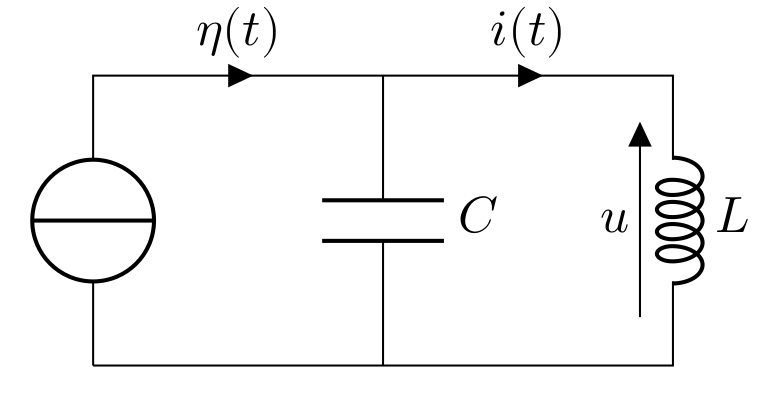
\includegraphics[width=\linewidth]{lc_energie}
\end{minipage}

\QR{Exprimer $\DS \dv{\Ec_{\rm tot}}{t}$ en fonction de $i$ et $\DS
\dv{i}{t}$.
}{
    Une fois le générateur de courant stoppé, l'énergie totale est la somme de
    l'énergie stockée dans le condensateur et de celle stockée dans la bobine,
    soit
    \[\Ec_{\rm tot} = \frac{1}{2}Cu^2 + \frac{1}{2}Li^2\]
    En dérivant on a donc
    \[ \dv{\Ec_{\rm tot}}{t} = \frac{1}{2}C\times 2u \dv{u}{t} +
        \frac{1}{2}\times 2i \dv{i}{t}\]
    Comme on demande de ne faire apparaître que $i$ dans le résultat, on
    remplace $u$ avec la relation courant-tension de la bobine et on développe~:
    \begin{align*}
        \dv{\Ec_{\rm tot}}{t} &= \frac{1}{2}C \times 2L \dv{i}{t} \dv{}{t} \left(
        L \dv{i}{t}\right) + \frac{1}{2} L\times 2i \dv{i}{t}\\
        \Leftrightarrow
        \dv{\Ec_{\rm tot}}{t} &= L^2C \dv{i}{t} \dv[2]{i}{t} + Li \dv{i}{t}\\
        \Leftrightarrow
        \Aboxed{\dv{\Ec_{\rm tot}}{t} &= L \dv{i}{t} \left( LC \dv[2]{i}{t} + i
        \right)}
    \end{align*}
}

\QR{Justifier qualitativement que $\Ec_{\rm tot}$ est constante. En
déduire l'équation différentielle vérifiée par $i$.
}{
    Le circuit ne compte qu'une bobine et un condensateur qui stockent de
    l'énergie sans la dissiper, et donc aucune résistance. L'énergie électrique
    dans le circuit est donc constante, et on en déduit qu'$\forall t \in
    \Rb^+$~:
    \begin{equation*}
        \dv{\Ec_{\rm tot}}{t} = 0
        \qdonc 
        L \dv{i}{t} \left( LC \dv[2]{i}{t} + i \right) = 0
    \end{equation*}
    On a donc un produit qui est nul. Or, la tension de la bobine $L \dv{i}{t}$
    ne peut être constamment nulle, c'est donc le terme entre parenthèses qui
    est nul, c'est-à-dire~:
    \begin{equation*}
        LC \dv[2]{i}{t} + i = 0
        \Longleftrightarrow
        \boxed{ \dv[2]{i}{t} + \w_0{}^2i = 0} \qavec \boxed{\w_0 =
        \frac{1}{\sqrt{LC}}}
    \end{equation*}
}

\QR{Retrouver cette équation par application des lois des nœuds et des
mailles.
}{
    $C$ et $L$ sont en parallèle, donc partagent la même tension $u$. Soit $i_C$
    le courant traversant $C$. Comme $\eta(t\geq0) = 0$, la loi des nœuds donne
    \[0 = i_C + i\qdonc C\dv{u}{t} + i = 0\]
    avec la RCT du condensateur. Comme $u$ est aussi la tension de $L$, avec la
    RCT de la bobine on retrouve bien
    \begin{equation*}
        \boxed{LC \dv[2]{i}{t} + i = 0}
    \end{equation*}
}

\QR{Établir les conditions initiales sur $i$ et sa dérivée.
}{
    À $t=0^-$, le circuit est alimenté par $\eta = I_0$ et on suppose le régime
    permanent atteint~: la bobine est donc équivalente à un fil, et le
    condensateur à un interrupteur ouvert. On en déduit donc
    \[i(0^-) = I_0 \qet u(0^-) = 0\]
    Par continuité de $i$ traversant la bobine et de $u$ aux bornes du
    condensateur, on a
    \[ \boxed{i(0^-) = i(0^+) = I_0} \qet u(0^-) = u(0^+) = 0\]
    Or, $u(0^+) = L \dv{i}{t} (0^+)$ d'après la RCT de la bobine. La seconde
    condition initiale est donc
    \[ \boxed{ \dv{i}{t} (0^+) = 0}\]
}

\QR{En déduire l'expression de $i(t)$.
}{
    L'équation étant homogène, la solution générale s'écrit
    \[ i(t) = A\cos(\w_0t) + B\sin(\w_0t)\]
    Avec la première CI, on a
    \[ i(0) = I_0 = A\]
    et avec la seconde on a
    \begin{gather*}
        \dv{i}{t} = -A\w_0\sin(\w_0t) + B\w_0\cos(\w_0t)\\
        \Rightarrow
        \dv{i}{t} (0) = \w_0B = 0\qdonc B = 0
    \end{gather*}
    Finalement, on trouve sans surprise
    \begin{equation*}
        \boxed{i(t) = I_0\cos(\w_0t)}
    \end{equation*}
}

\resetQ
\section{Étude énergétique d'un oscillateur amorti électrique}

\begin{minipage}{0.7\linewidth}
    Un circuit électrique est composé d'une résistance $R$, d'une bobine
    d'inductance $L$ et d'un condensateur de capacité $C$. Ces dipôles sont
    disposés en série et on soumet le circuit à un échelon de tension tel que~: 
    $ \left\{
            \begin{array}{rcl}
                e(t<0)    & = & 0 \\
                e(t\geq0) & = & E
            \end{array}
    \right.$.  On pose $\gamma = \dfrac{R}{2L}$ et $\w_0 = \dfrac{1}{\sqrt{LC}}$
\end{minipage}
\begin{minipage}{0.3\linewidth}
    \centering
    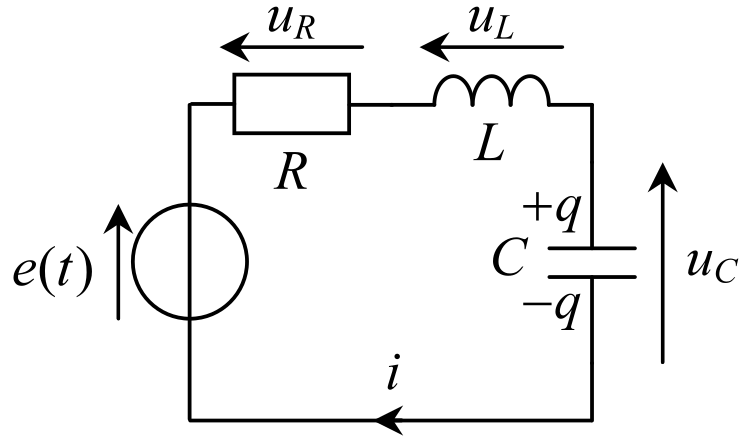
\includegraphics[width=\linewidth]{rlc_energie}
\end{minipage}

\QR{Expliquer simplement pourquoi à $t = 0^-$ la charge $q$ et le courant
$i$ sont nuls.
}{
    À $t=0^-$, le circuit est depuis longtemps sous la tension $e=0$~; il a donc
    atteint son régime permanent, et le condensateur s'est déchargé et est
    équivalent à un interrupteur ouvert~: forcément,
    \begin{equation*}
        \boxed{i(0^-) = 0} \qet \boxed{q(0^-) = Cu(0^-) = 0}
    \end{equation*}
}

\QR{Montrer que l'équation différentielle vérifiée par la charge $q(t)$ du
    condensateur pour $t > 0$ est~:
    \[ \dv[2]{q}{t} + 2\gamma \dv{q}{t} + \w_0{}^2 q = \frac{E}{L}\]
    Préciser, en les justifiant, les valeurs initiales de la
    charge $q(0^+)$ et de sa dérivée.
}{
    Avec une loi des mailles, les RCT de la résistance, de la bobine et du
    condensateur et la relation $i = \dv{q}{t}$, on a
    \begin{gather*}
        u_L + u_R + u_C = E
        \Leftrightarrow
        L \dv{i}{t} + Ri + \frac{q}{C} = E\\
        \Leftrightarrow
        L \dv[2]{q}{t} + R \dv{q}{t} + \frac{q}{C} = E
        \Leftrightarrow
        \dv[2]{q}{t} + 2\gamma \dv{q}{t} + \frac{q}{C} = \frac{E}{L}
    \end{gather*}
    Concernant les conditions initiales, la tension aux bornes d'un condensateur
    est continue donc sa charge aussi, c'est-à-dire
    \[\boxed{q(0^-) = q(0^+) = 0}\]
    et comme le courant traversant une bobine est également continu, on a
    \[i(0^-) = i(0^+) = 0\qsoit \boxed{ \dv{q}{t} (0^+) = 0}\]
}

Le circuit présente différents régimes suivant les valeurs de $R$, $L$ et $C$.
On suppose dans la suite la condition $\w_0 > \gamma$ réalisée.

\QR{Montrer que l'expression de la charge pour $t > 0$ peut se mettre sous la
    forme
    \[q(t) = [A \cos(\w t) + B \sin(\w t)] \exr^{−\gamma t} + D\]
    avec $A$, $B$ et $D$ des constantes à exprimer en fonction de $C$, $E$,
    $\w_0$ et $\gamma$.
}{

    L'équation caractéristique de discriminant $\Delta$ de l'équation homogène
    est
    \[r^2 + 2\gamma r + \w_0{}^2 = 0 \Rightarrow \Delta = 4(\gamma^2
    -\w_0{}^2)\]
    Comme $\w_0 > \gamma$, on a $\Delta <0$ et on est donc dans un régime
    pseudo-périodique. On aura donc
    \begin{gather*}
        r_\pm = -\frac{\cancel{2}\gamma}{\cancel{2}} \pm \Ir
            \frac{1}{\bcancel{2}}\sqrt{\bcancel{4}(\w_0{}^2 - \gamma^2)}
        \Leftrightarrow
        \boxed{r_\pm = -\gamma \pm \Ir \w}
            \qavec
        \boxed{\w = \sqrt{\w_0{}^2 - \gamma^2}}
    \end{gather*}
    La solution particulière est $\frac{E}{L\w_0{}^2} = CE$, donc on aura la forme
    générale
    \begin{equation*}
        \boxed{q(t) = \exr^{-\gamma t} \left( A\cos\wt + B\sin\wt \right) +
        CE}
    \end{equation*}
    Avec la première CI,
    \[q(0) = A+CE = 0 \Leftrightarrow \boxed{A = -CE}\]
    et avec la seconde,
    \[\dv{q}{t} (0) = -\gamma A + B\w = 0
      \Leftrightarrow
      \boxed{B = -CE \frac{\g}{\sqrt{\w_0{}^2 - \g^2}}}\]
    soit finalement
    \begin{equation*}
        \boxed{q(t) = CE -
            CE \exr^{-\gamma t}
            \left( \cos\wt +
                \frac{\g}{\sqrt{\w_0{}^2 - \g^2}}\sin\wt
            \right)}
    \end{equation*}
}

\QR{Exprimer le courant $i(t)$ dans le circuit pour $t > 0$ en fonction de
$C$, $E$, $\w_0$ et $\gamma$.
}{
    On dérive $q$~:
    \begin{equation*}
        \boxed{i(t) = CE \frac{\w_0{}^2}{\w}\exr^{-\g t}\sin\wt}
    \end{equation*}
}

\QR{Donner l'allure des courbes $q(t)$ et $i(t)$. Quelles sont leurs valeurs à
    la fin du régime transitoire~? Justifier par des considérations simples ces
    valeurs atteintes.
}{
    La charge finale atteinte est $CE$ et le courant final est nul. Ces valeurs
    se retrouvent facilement en remarquant qu'en régime permanent, le
    condensateur se comporte comme un interrupteur ouvert et la bobine comme un
    fil~; le courant est alors nul, et ainsi les tensions aux bornes de $L$ et
    $R$ le sont également~: la tension $E$ du circuit est entièrement dans
    $u_C$, et sa charge est donc $CE$.
    \begin{center}
        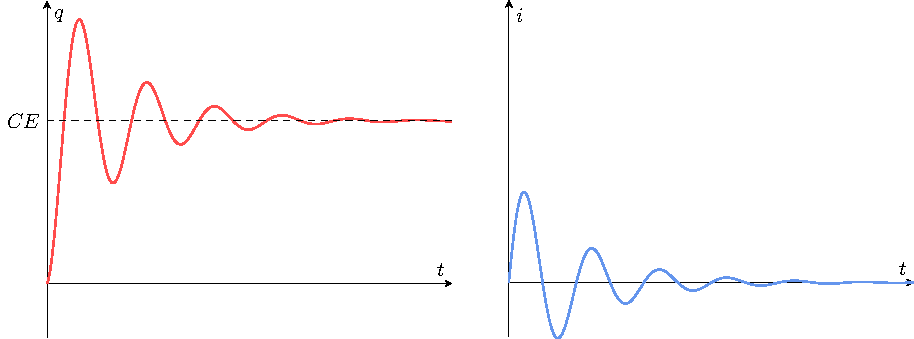
\includegraphics[width=\linewidth]{energ_amorti-qi}
    \end{center}
}

\QR{Déterminer l'énergie totale $\Ec_G$ fournie par le générateur ainsi que
    l'énergie $\Ec_{LC}$ emmagasinée dans la bobine et le condensateur à la fin
    du régime transitoire en fonction de $C$ et $E$. En déduire l'énergie
    dissipée par effet \textsc{Joule} dans la résistance. Ces résultats
    dépendent-ils du régime particulier dans lequel se trouve le circuit~?
    Interpréter le résultat paradoxal qui apparaît dans le cas limite $R
    \longrightarrow 0$.
}{  
    Un bilan de puissance sur le circuit, (i.e.\ \textbf{loi des mailles$\times
    i$}) donne
    \[ \Pc_L + \Pc_C + \Pc_J = \Pc_G \Rightarrow \boxed{\Ec_{LC} + \Ec_J = \Ec_G}\]
    On trouve donc naturellement que l'énergie du générateur se répartit entre
    la bobine, l'inductance et la résistance. On va donc déterminer $\Ec_G$ et
    $\Ec_{LC}$ pour trouver $\Ec_J$ par différence.\bigbreak
    L'énergie fournie par le générateur s'obtient en intégrant la puissance
    fournie $Ei$ par le générateur entre $t=0$ et $t \rightarrow \infty$. En se
    rappelant que $i = \dv{q}{t}$, cette intégrale se ramène à une simple
    intégration sur $q$ de valeur initiale 0 et de valeur finale $CE$~:
    \[ \Ec_G = \int_{0}^{\infty} Ei \dt = \int_{0}^{CE} E\dd q = E \left[
    q \right]^{q=0}_{q=CE} \Leftrightarrow \boxed{\Ec_G = CE^2}\]
    L'énergie $\Ec_{LC}$ emmagasinée par l'inductance et la capacité se calcule
    par différence des énergies stockées dans ces dipôles entre l'instant final
    et l'instant initial. Or, les deux dipôles sont initialement déchargés, et
    comme $i = 0$ à la fin l'énergie de la bobine est nulle. Ainsi,
    \[\Ec_{LC} = \left[ \frac{1}{2}Li(t)^2 + \frac{1}{2} \frac{q(t)^2}{C}
    \right]_{t=0}^{t=\infty} \Leftrightarrow \boxed{\Ec_{LC} = \frac{1}{2}CE^2}\]
    Ainsi,
    \[ \Ec_{J} = \Ec_G - \Ec_{LC} \Leftrightarrow \boxed{\Ec_J =
    \frac{1}{2}CE^2}\]
    Ces calculs sont indépendants du régime dans lequel se trouve le circuit.
    L'énergie fournie par le générateur est deux fois plus grande que celle
    stockée par la bobine et le condensateur, \textbf{indépendamment de la
    valeur de la résistance du circuit}.\smallbreak
    Extrapolé à $R \longrightarrow 0$, ce résultat semble contredire le
    principe de conservation de l'énergie, puisque la seconde moitié d'énergie
    ne peut plus être dissipée par effet \textsc{Joule}. En fait, pour $R
    \longrightarrow 0$, le circuit oscille de façon sinusoïdale~: on n'atteint
    jamais de régime permanent continu, et la bobine et le condensateur stockent
    et restituent alternativement de l'énergie.
}

\resetQ
\section{Circuit de \textsc{Wien}}

\begin{minipage}{0.60\linewidth}

    On réalise le montage suivant. On ferme l'interrupteur à l'instant $t =0$,
    $C$ traversé par $i'$ étant initialement chargé et $C$ traversé par $i$
    étant initialement déchargé.\smallbreak
    On pose $\tau = RC$. Données~: $R = \SI{10}{k\ohm}$ et $C = \SI{0.1}{\micro
    F}$.
\end{minipage}
\begin{minipage}{0.40\linewidth}
    \centering
    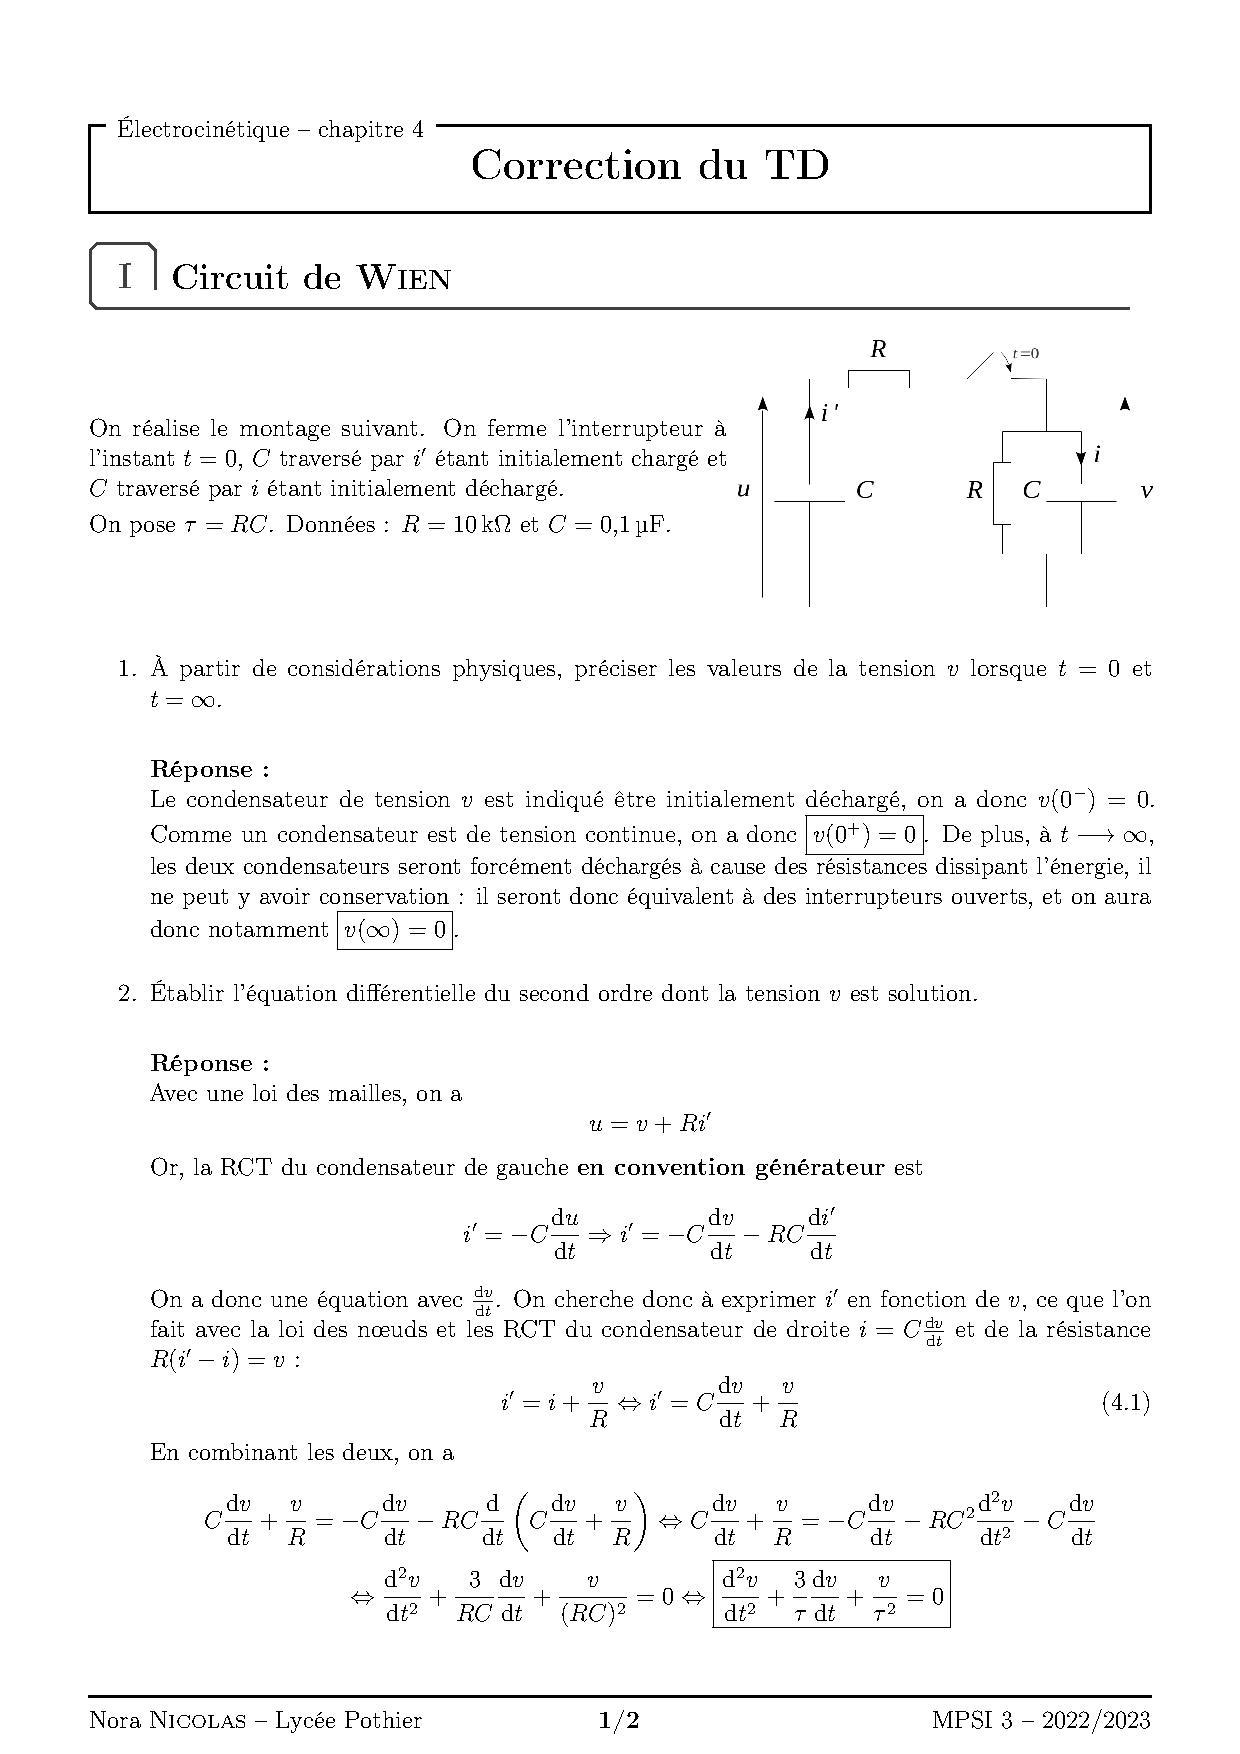
\includegraphics[width=\linewidth]{wien}
\end{minipage}

\QR{À partir de considérations physiques, préciser les valeurs de la tension $v$
    lorsque $t = 0$ et $t = \infty$.
}{
    Le condensateur de tension $v$ est indiqué être initialement déchargé, on a
    donc $v(0^-) = 0$. Comme un condensateur est de tension continue, on a donc
    \fbox{$v(0^+) = 0$}. De plus, à $t \longrightarrow \infty$, les deux
    condensateurs seront forcément déchargés à cause des résistances dissipant
    l'énergie, il ne peut y avoir conservation~: il seront donc équivalent à des
    interrupteurs ouverts, et on aura donc notamment \fbox{$v(\infty) = 0$}.
}

\QR{
    Établir l'équation différentielle du second ordre dont la tension $v$ est
    solution.
}{
    Avec une loi des mailles, on a
    \[ u = v+Ri'\]
    Or, la RCT du condensateur de gauche \textbf{en convention générateur} est
    \[i' = -C \dv{u}{t} \Rightarrow i' = -C \dv{v}{t} - RC \dv{i'}{t}\]
    On a donc une équation avec $\dv{v}{t}$. On cherche donc à exprimer $i'$ en
    fonction de $v$, ce que l'on fait avec la loi des nœuds et les RCT du
    condensateur de droite $i = C \dv{v}{t}$ et de la résistance $R(i'-i) = v$~:
    \begin{equation}\label{eq:wieni}
        i' = i + \frac{v}{R} \Leftrightarrow i' = C \dv{v}{t} + \frac{v}{R}
    \end{equation}
    En combinant les deux, on a
    \begin{gather*}
        C \dv{v}{t} + \frac{v}{R} =
            -C \dv{v}{t} - RC \dv{}{t} \left( C \dv{v}{t} + \frac{v}{R} \right)
        \Leftrightarrow
        C \dv{v}{t} + \frac{v}{R} =
            -C \dv{v}{t} - RC^2 \dv[2]{v}{t} - C \dv{v}{t}\\
        \Leftrightarrow
        \dv[2]{v}{t} + \frac{3}{RC} \dv{v}{t} + \frac{v}{(RC)^2} = 0
        \Leftrightarrow
        \boxed{\dv[2]{v}{t} + \frac{3}{\tau} \dv{v}{t} + \frac{v}{\tau^2} = 0}
    \end{gather*}
}

\QR{
    En déduire l'expression de $v(t)$ sans chercher à déterminer les
    constantes d'intégration.
    
}{
    On écrit l'équation caractéristique de discriminant $\Delta$~:
    \begin{gather*}
        r^2 + \frac{3}{\tau}r + \frac{1}{\tau^2} = 0 \Rightarrow \Delta =
        \frac{9}{\tau^2} - \frac{4}{\tau^2} = \frac{5}{\tau^2} > 0\\
        \Longrightarrow r_\pm = - \frac{3}{2\tau} \pm \frac{\sqrt{5}}{2\tau} < 0
    \end{gather*}
    On a donc un régime apériodique, dont les solutions générales sont
    \[\boxed{v(t) = A\exr^{r_+t} + B\exr^{r_-t}}\]
}

\QR{Donner l'allure du graphe correspondant à $v(t)$. 
}{
    \begin{minipage}{0.49\linewidth}

        Le condensateur est initialement chargé. Soit $E$ sa tension initiale.
        On utilise l'équation~\ref{eq:wieni} pour trouver que $\dv{v}{t} (0) =
        \frac{i' (0)}{C}$, sachant qu'à $t = 0$ le circuit est équivalent à un
        circuit $RC$ en décharge et qu'on a donc $i'(0) = E/R$. On trouve ainsi
        \[\boxed{\dv{v}{t} (0) = \frac{E}{\tau}}\]
        En finissant la détermination des constantes d'intégration, on trouve
        \begin{equation*}
            \boxed{v(t) = \frac{E}{\tau(r_+ - r_-)}
                          \left[ \exr^{r_+t} - \exr^{r_-t} \right]}
        \end{equation*}
        \hfill
    \end{minipage}
    \begin{minipage}{0.49\linewidth}
        \begin{center}
            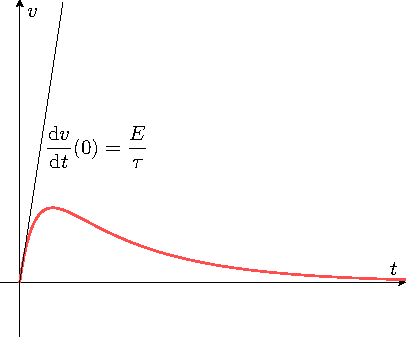
\includegraphics[width=\linewidth]{wien_carac}
        \end{center}
    \end{minipage}
}

\end{document}
